\section{Experimental Results}
\label{section:experimental-results}

\begin{figure*}[ht]
  \subfigure[\emph{Pillar scenario} with randomly moving goal object\label{figure:learning_rate_pillar_dirchange}]{\includegraphics[width=0.24\textwidth]{plot_quality_learning-pillardir.eps}}\hfill\subfigure[\emph{Pillar scenario} with intelligent goal object\label{figure:learning_rate_pillar_intelligent}]{\includegraphics[width=0.24\textwidth]{plot_quality_learning-pillarint.eps}}\hfill\subfigure[\emph{Random scenario} with intelligent goal object\label{figure:learning_rate_random_intelligent}]{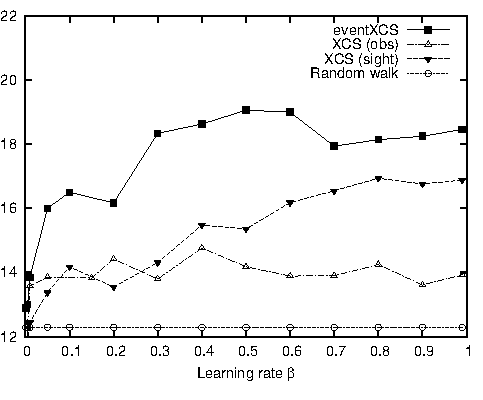
\includegraphics[width=0.24\textwidth]{plot_quality_learning-randint.eps}}\hfill\subfigure[\emph{Difficult scenario} with goal object moving only into one direction\label{figure:learning_rate_difficult}]{\includegraphics[width=0.24\textwidth]{plot_quality_learning-difficult.eps}}\caption{\mathversion{bold}Comparison of different values for the learning rate $\beta$ for different XCS variants}\label{figure:learning_rate}
\end{figure*}

%\begin{figure*}[ht]
%  \subfigure[Comparison of different \emph{maxStackSize} values for SXCS in different scenarios\label{figure:max-stack-size}]{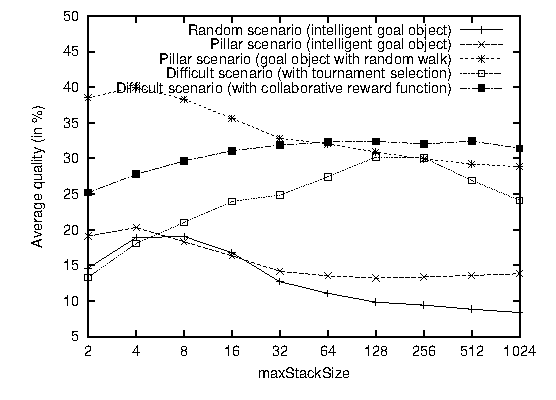
\includegraphics[width=0.32\textwidth]{plot_quality_maxstacksize.eps}}\hfill\subfigure[Comparison of the average quality over time in the \emph{difficult scenario}\label{figure:experiment-difficult}]{\includegraphics[width=0.32\textwidth]{plot_average_last_x_steps_goal_agent_observed-difficult.eps}}\caption{\mathversion{bold}Comparison of different XCS variants}\label{figure:learning_rate2}
%\end{figure*}

\begin{figure*}[ht]
  \subfigure[\emph{Pillar scenario} with randomly moving goal object\label{figure:experiment-pillardir}]{\includegraphics[width=0.24\textwidth]{plot_average_last_x_steps_goal_agent_observed-pillardir.eps}}\hfill\subfigure[\emph{Pillar scenario} with intelligent goal object\label{figure:experiment-pillarint}]{\includegraphics[width=0.24\textwidth]{plot_average_last_x_steps_goal_agent_observed-pillarint.eps}}\hfill\subfigure[\emph{Random scenario} with intelligent goal object\label{figure:experiment-randint}]{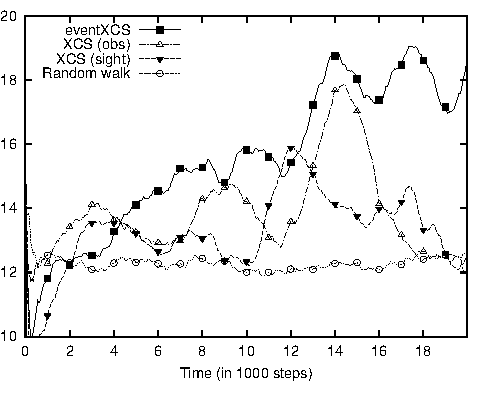
\includegraphics[width=0.24\textwidth]{plot_average_last_x_steps_goal_agent_observed-randint.eps}}\hfill\subfigure[\emph{Difficult scenario} with goal object moving only in one direction\label{figure:experiment-difficult}]{\includegraphics[width=0.24\textwidth]{plot_average_last_x_steps_goal_agent_observed-difficult.eps}}\caption{\mathversion{bold}Comparison of the average quality over time of different XCS variants}\label{figure:experiments}
\end{figure*}

Many different combinations of the reward function adaptions discussed above are possible. The main goal of this paper is to show that there are better implementations than XCS, not to find the best possible implementation. Therefore, this paper concentrates on the comparison of the XCS variants presented in the following Section~\ref{subsection:xcs-variants}.

In order to properly compare them it was important to determine good parameter settings for each variant. While most of the standard values given in~\cite{BW02} (``Commonly Used Parameter Settings'') showed good results, some special settings need closer examination. Although thousands of different combinations were tested, the parameter discussion is not necessarily complete. Of main importance was that any score below the algorithm with randomized movements has to be dismissed as it is difficult to say if a parameter settings with better results (below the result of the random algorithm) just makes the agent move more randomly or if it actually learns better. The results of the parameter discussion is described in Section~\ref{subsection:xcs-parameters}. Finally, in the subsequent Section~\ref{subsection:experimental_results}, the results of a number of experiments are presented.

\subsection{XCS Variants}
\label{subsection:xcs-variants}

Many different combinations of the reward function options discussed in Section~\ref{section:the-reward-function} are possible. Surprisingly no reward function option on its own showed a better performance. Using the collaborative environmental reward function from Section~\ref{subsection:environment-reward-function} even reduced the performance significantly. The best results showed a standard implementation of XCS with an environmental reward function that returns $1$ when the goal object is in observation range and $0$ at all other times. This will be referred to as ``{\bf XCS}''.

Using events (see Section~\ref{subsection:events}) in combination with the reward distribution based on the generated events (see Section~\ref{subsection:reward-distribution}) showed in some scenarios significant better performance than any of the other XCS variants. In addition it is able to perform well with any of the tested environmental reward functions while XCS only works with a reward function modeled after the global goal. This will be referred to as ``{\bf SXCS}'' (\emph{Supervising eXtended Classifier System}).


\subsection{XCS/SXCS Parameters}
\label{subsection:xcs-parameters}

The parameter \emph{maxStackSize} that was introduced in section~\ref{subsection:events} determines when the stack overflows and a neutral event occurs. While further research is required, a relatively good value was determined by several experiments. Similar to XCS' prediction discount parameter $\gamma$ the optimal value is a compromise between several conflicting factors: Larger values result in an inclusion of older - maybe irrelevant - actions in the reward of positive or negative events. Smaller values can reduce the delay between an event and the actual reward but they may also lead to a possible disregard of actions that were important in achieving the current event. As Figure~\ref{figure:max-stack-size} shows the optimal value depends on the complexity of the scenario. For comparison in all tests a value of $8$ will be used.

%value does not have a large impact in the \emph{pillar} or \emph{random scenario}, only at around \emph{maxStackSize}~\( = 8\) a difference can be seen. The \emph{difficult scenario} on the other hand favors a larger value (\emph{maxStackSize}~\( = 32\)). In conclusion more complex routes to the goal probably require a larger value for \emph{maxStackSize}.

%\subsection{Learning rate $\beta$}\label{subsection:learning_rate}

During the tests another important parameter was the learning rate $\beta$. In a similar type of scenario in~\cite{1102281} a value below the standard value was proposed (\(\beta = 0.02\)). The reason was that dynamic multi-agent systems can be described only by movement probabilities so the learning process has to be slow and careful. Tests (see Figure~\ref{figure:learning_rate}) showed an optimal value between \(0.01\) and \(0.5\) depending on the scenario. Very low values seem to always harm the learning process while larger values seem to harm the learning process in some scenarios while improving it in others (see Figure~\ref{figure:learning_rate_difficult}). To maintain comparability between the scenarios and to other implementations of XCS a value of \(0.05\) was used for $\beta$ in further tests. According to~\cite{BW02} the maximum number of classifiers $N$ should be chosen big enough so that \emph{covering} happens only in the beginning of a run. For the scenario in question tests have shown that a population size of around $512$ fulfils this criteria. The classifier sets were filled with random classifiers~\cite{Butz2006} but no significant difference was seen. Instead sometimes a slower convergence was observed, probably because the corresponding system had to unlearn irrelevant classifiers. The \emph{GA threshold} parameter $\theta_{\mathrm{GA}}$ was set to $25$, larger values seemed to reduce the quality of the algorithm. As SXCS itself does use the quadratic reward distribution, the parameter \emph{reward prediction discount} $\gamma$ is only needed to compare XCS with SXCS. Tests have been inconclusive so the standard value of \(\gamma = 0.71\) was used. Only \(\gamma = 1.0\) showed significant different results in some cases. It seems that while a reduction of the transfer of the reward is needed, the actual value is of little importance. Other parameters, like the subsumption threshold $\theta_{\mathrm{sub}}$, GA threshold $\theta_{\mathrm{GA}}$ and the mutation probability $\mu$ values in the standard range were used ($20.0$, $25.0$ and $0.05$ respectively).



%Table~\ref{table:lcs-parameter} shows the special settings that were used.

%\begin{table}[ht]
%\caption{Used parameter values and standard values}
%\centering
%\begin{tabular}{c c c}
%\hline\hline
%Parameter & Value & Standard (see~\cite{BW02})\\ [0.5ex]
%\hline
%max population \(N\) & \textbf{512} & [-]\\
%subsumption threshold \(\theta_{\mathrm{sub}}\) & 20.0 & [20.0+]\\
%GA threshold \(\theta_{\mathrm{GA}}\) & 25 & [25-50]\\
%mutation probability \(\mu\) & \(0.05\) & [0.01-0.05]\\
%reward prediction discount \(\gamma\) & 0.71 & [0.71]\\
%learning rate \(\beta\) & \textbf{0.05} & [0.1-0.2]\\
%tournament factor & 0.84 & [-]\\ [0.5ex]
%\hline
%\end{tabular}
%\label{table:lcs-parameter}
%\end{table}

\subsection{Experimental results}\label{subsection:experimental_results}

%Figure~\ref{figure:experiment-heuristics} show a comparison between possible static strategies. Collaborative strategies have just a small advantage over simple greedy strategies.



Figure~\ref{figure:experiment-pillardir}, Figure~\ref{figure:experiment-pillarint} and Figure~\ref{figure:experiment-randint} show the average percentage of time steps where the goal object was in observation range (each averaged over the last 2000 steps). With an intelligent goal object SXCS clearly outperforms XCS, while in the case with the randomly moving goal object both variants show a similar learning curve. In all cases increasing the base reward function for XCS from observation range to sight range resulted in worse results.\\
The case with a randomly moving (but obstacle-evading) goal object in the \emph{random scenario} is not displayed, none of the XCS variants are able to gain a significant advantage over a ``random walk'' strategy.

%\begin{figure}[ht]
%\centerline{	
%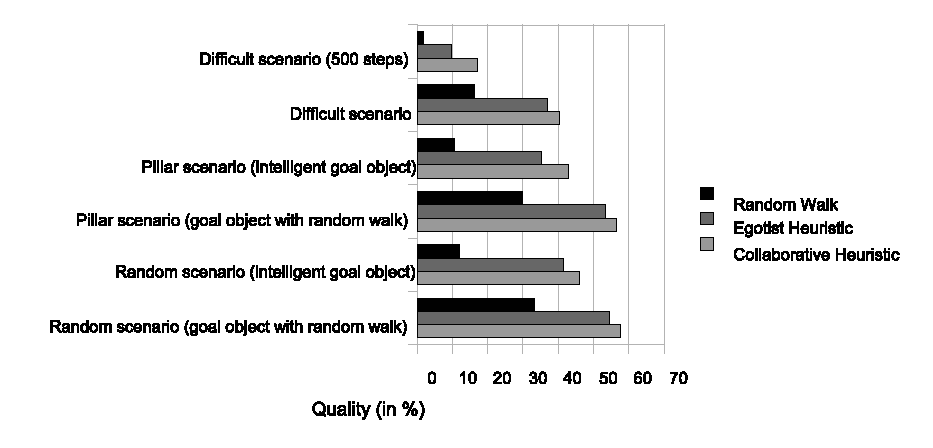
\includegraphics[scale=0.6]{experiment_heuristics.eps}
%}
%\caption{Comparison of different static strategies}
%\label{figure:experiment-heuristics}
%\end{figure}




%\begin{figure}[ht]
%\centerline{	
%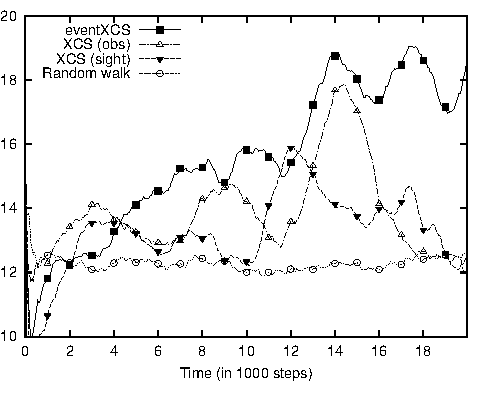
\includegraphics{plot_average_last_x_steps_goal_agent_observed-randint.eps}
%}
%\caption{\emph{Random scenario} with intelligent goal object}
%\label{figure:experiment-randint}
%\end{figure}

%\begin{figure}[ht]
%\centerline{	
%\includegraphics{plot_average_last_x_steps_goal_agent_observed-pillarint.eps}
%}
%\caption{\emph{Pillar scenario} with intelligent goal object}
%\label{figure:experiment-pillarint}
%\end{figure}

%\begin{figure}[ht]
%\centerline{	
%\includegraphics{plot_average_last_x_steps_goal_agent_observed-pillardir.eps}
%}
%\caption{\emph{Pillar scenario} with randomly moving goal object}
%\label{figure:experiment-pillardir}
%\end{figure}

%\subsection{Comparison in the Pillar Scenario}
%\label{subsection:xcs-pillar-scenario}
%\begin{figure}[ht]
%\centerline{	
%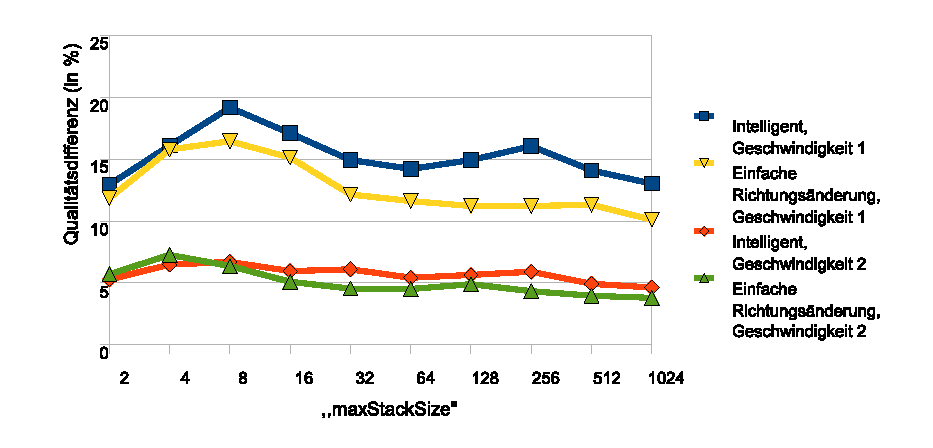
\includegraphics[scale=0.6]{experiment_pillar_scenario.eps}
%}
%\caption{Comparison of different XCS variants in the pillar scenario}
%\label{figure:experiment-pillar-scenario}
%\end{figure}
%See Figure~\ref{figure:experiment-pillar-scenario}
%\subsection{Comparison in the Random Scenario}
%\label{subsection:xcs-random-scenario}
%TODO
%\begin{figure}[ht]
%\centerline{	
%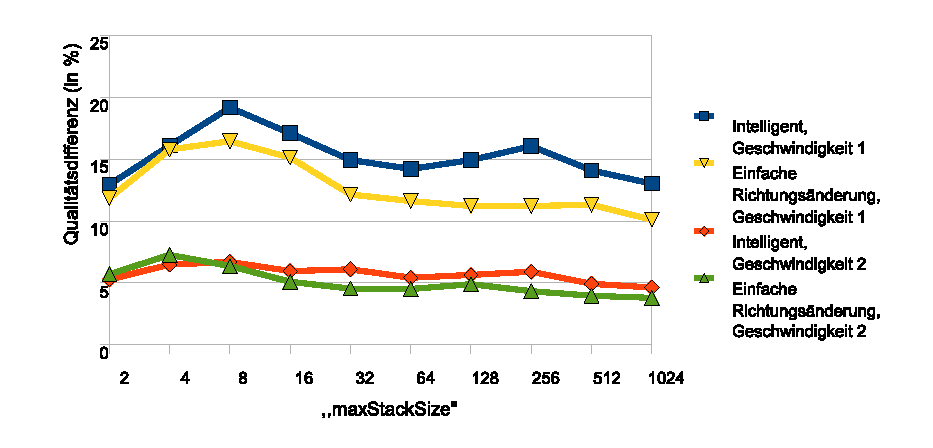
\includegraphics[scale=0.6]{experiment_random_scenario.eps}
%}
%\caption{Comparison of different XCS variants in the random scenario}
%\label{figure:experiment-random-scenario}
%\end{figure}
%See Figure~\ref{figure:experiment-random-scenario}

%\subsection{Comparison in the \emph{Difficult Scenario}}
%\label{subsection:xcs-difficult-scenario}

In the \emph{difficult scenario} SXCS clearly fails (see Figure~\ref{figure:learning_rate_difficult}). Alternative implementations of SXCS with \emph{tournament selection} on the other hand solve the problem but reach only a lower level as XCS with \emph{best selection} (see Figure~\ref{figure:experiment-difficult}). But as in the \emph{random scenario} with an intelligent goal object XCS seems to have problems with overlearning. Increasing the learning rate $\beta$ to $0.2$ increase the quality in short-term, but in long-term XCS still has problems while SXCS present a very stable learning curve. In connection with a collaborative base reward function SXCS is even able to outperform XCS in the long run.\\
